% Untangling Federal Jurisdiction
% Part 1 of 3

% All content comes from Stephen Pratt. I have no idea if he approves of this effort or not.

\documentclass{beamer}
\usetheme{Madrid}
%\usetheme{Goettingen}
\usefonttheme{serif}
\usefonttheme{structuresmallcapsserif}
% \usepackage[font=small,labelfont=bf]{caption}
\usepackage{xcolor}
\usepackage{rotating}

\setbeamerfont{section title}{parent=title}
\setbeamercolor{section title}{parent=titlelike}
\defbeamertemplate*{section page}{default}[1][]
{
    \centering
    \begin{beamercolorbox}[sep=8pt,center,#1]{section title}
        \usebeamerfont{section title}\insertsection\par
    \end{beamercolorbox}
}
\newcommand*{\sectionpage}{\usebeamertemplate*{section page}}

\def\Put(#1,#2)#3{\leavevmode\makebox(0,0){\put(#1,#2){#3}}}

\makeatletter
\setbeamertemplate{footline}
{
    % Commented out to remove footer line entirely
%    \leavevmode%
%    \hbox{%
%    \begin{beamercolorbox}[wd=.333333\paperwidth,ht=2.25ex,dp=1ex,center]{author in head/foot}%
%        \usebeamerfont{author in head/foot}\insertshortauthor%~~\beamer@ifempty{\insertshortinstitute}{}{(\insertshortinstitute)}
%    \end{beamercolorbox}%
%    \begin{beamercolorbox}[wd=.333333\paperwidth,ht=2.25ex,dp=1ex,center]{title in head/foot}%
%        \usebeamerfont{title in head/foot}\insertshorttitle
%    \end{beamercolorbox}%
%    \begin{beamercolorbox}[wd=.333333\paperwidth,ht=2.25ex,dp=1ex,right]{date in head/foot}%
%        \usebeamerfont{date in head/foot}\insertshortdate{}\hspace*{2em}
%        \insertframenumber{} / \inserttotalframenumber\hspace*{2ex} 
%    \end{beamercolorbox}}%
%    \vskip0pt%
}
\makeatother

\newenvironment<>{varblock}[2][\textwidth]{
    \begin{center}
        \begin{minipage}{#1}
            \setlength{\textwidth}{#1}
            \begin{actionenv}#3
                \def\insertblocktitle{#2}
                \par
                \usebeamertemplate{block begin}}
            {\par
                \usebeamertemplate{block end}
            \end{actionenv}
        \end{minipage}
    \end{center}
}

\DeclareGraphicsExtensions{.pdf,.png,.jpg}


\begin{document}

\title[Untangling Federal Jurisdiction]{Untangling Federal Jurisdiction Within a State}
\author{Stephen Pratt}

%\frame{\titlepage}

%\begin{frame}{Thomas Paine, 1737-1809}
%    \begin{columns}[c]
%        \column{2in}
%            \begin{figure}[h]
%                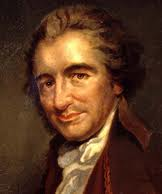
\includegraphics{img/thomas-paine.png}
%            \end{figure}
%        \column{1.5in}
%            "All power exercised over a nation must have some beginning.  It must either be delegated or assumed.  There are no other sources.  All delegated power is trust, and all assumed power is usurpation.  Time does not alter the nature and quality of either."
%    \end{columns}
%\end{frame}

%\begin{frame}{News Release}
%    \begin{block}{March 23, 2012}
%    SALT LAKE CITY - Today, Utah Governor Gary R. Herbert signed House Bill 148, which demands the federal government make good on the promises made in the 1894 Enabling Act to extinguish title to federal lands in Utah. 
%    \end{block}
%\end{frame}
%
%\begin{frame}{News Release}
%    \begin{block}{April 25, 2012}
%    WASHINGTON – Today, Senator Mike Lee responded to comments made yesterday by Interior Secretary Ken Salazar regarding recent Utah state land transfer legislation.
%    \end{block}
%\end{frame}

\section{A Recurrence to First Principles}

%\frame{\sectionpage}

%\begin{frame}
%    \begin{columns}[onlytextwidth]
%        \column{0.5\textwidth}
%            \centering
%            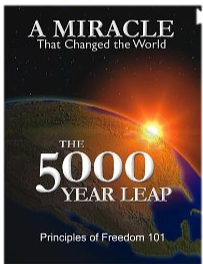
\includegraphics{img/5000-year-leap.png}
%            \\ 28
%        \column{0.5\textwidth}
%            \pause
%            \centering
%            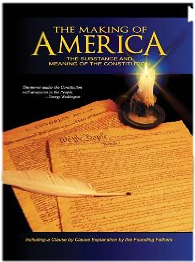
\includegraphics{img/making-of-america.png}
%            \\ 286
%    \end{columns}
%\end{frame}
%
%\begin{frame}{Blackstone's Law Dictionary}
%    \begin{columns}[onlytextwidth]
%        \column{0.5\textwidth}
%            \centering
%            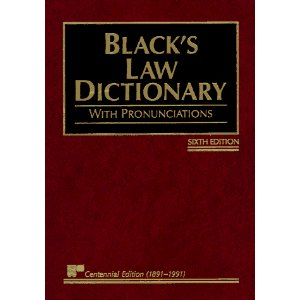
\includegraphics[width=0.75\textwidth]{img/blacks-law.png}
%            \\ { \tiny 1920 pages }
%        \column{0.5\textwidth}
%        \textbf{Jurisdiction} \\
%        Page 927 \\
%        1.  A government's general power to exercise authority over all persons and things within its territory;
%    \end{columns}
%\end{frame}
%
%\begin{frame}{Sheriff Gil Gilbertson}
%    \begin{columns}[onlytextwidth]
%        \column{0.5\textwidth}
%            \centering
%            Where does the United States Forest Service's authority come from?
%            \\ { \tiny October, 2011 }
%        \column{0.5\textwidth}
%            \centering
%            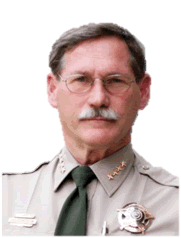
\includegraphics[width=0.75\textwidth]{img/gil-gilbertson.png}
%            \\ Sheriff Gil Gilbertson
%            \\ Josephine County, Oregon
%    \end{columns}
%\end{frame}
%
%\begin{frame}{Sheriff Glenn Palmer}
%    \begin{columns}[onlytextwidth]
%        \column{0.5\textwidth}
%            \centering
%            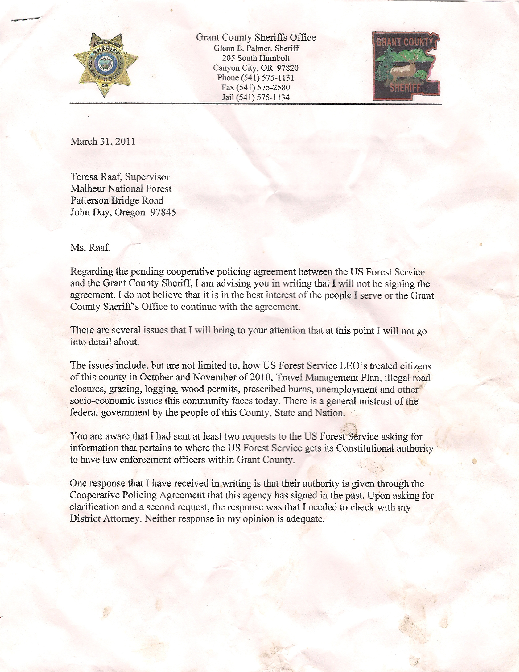
\includegraphics[width=0.75\textwidth]{img/glenn-palmer-letter.png}
%            \\ March 31, 2011
%        \column{0.5\textwidth}
%            \centering
%            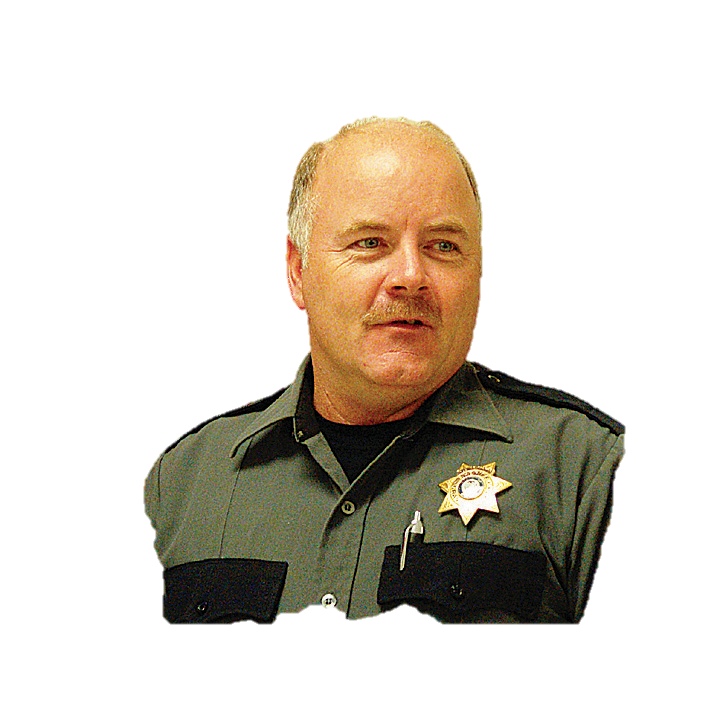
\includegraphics[width=0.75\textwidth]{img/glenn-palmer.png}
%            \\ Sheriff Glenn Palmer
%            \\ Grant County, Oregon
%    \end{columns}
%\end{frame}
%
%\begin{frame}{Sheriff Glenn Palmer}
%    \begin{columns}[onlytextwidth]
%        \column{0.5\textwidth}
%            \centering
%            { \Large Where does the United States Forest Service get its
%            \textbf{\emph{Constitutional}} authority to have law enforcement
%            officers in Grant County? }
%        \column{0.5\textwidth}
%            \centering
%            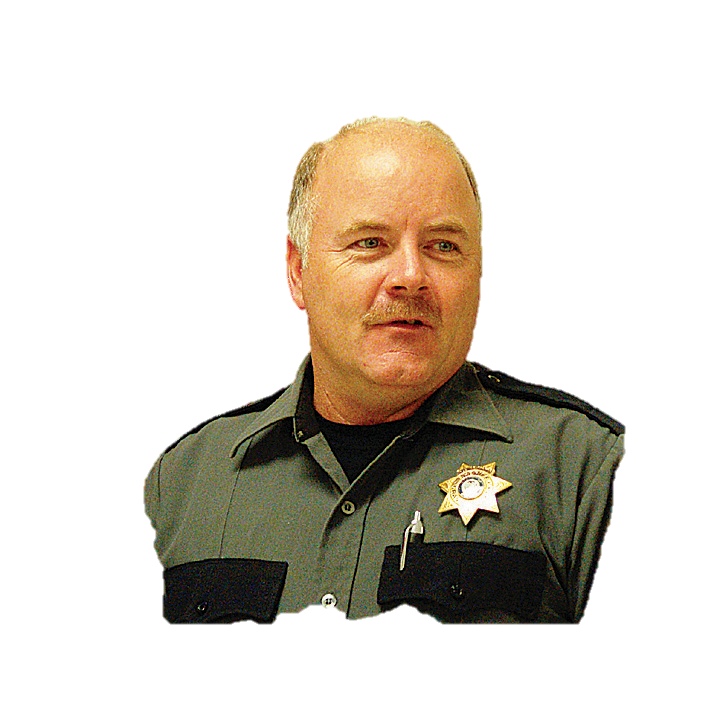
\includegraphics[width=0.75\textwidth]{img/glenn-palmer.png}
%            \\ Sheriff Glenn Palmer
%            \\ Grant County, Oregon
%    \end{columns}
%\end{frame}
%
%\begin{frame}{Portland, Oregon}
%    
\includegraphics[width=0.3\textwidth]{img/doj.png}
%    
\includegraphics[width=0.3\textwidth]{img/usfs.png}
%    
\includegraphics[width=0.3\textwidth]{img/ossa.png}
%    {   
%        \centering
%        \\ { \huge January 12, 2012 } \\
%    }
%\end{frame}
%
%\begin{frame}{Portland, Oregon}
%    \begin{columns}[onlytextwidth]
%        \column{0.5\textwidth}
%            \centering
%            
\includegraphics[height=0.28\textheight]{img/amanda-marshall.png}
%            \\ United States Attorney \\ S. Amanda Marshall \\
%            
\includegraphics[height=0.28\textheight]{img/elmer-dickens.png}
%            \\ Washington County Attorney \\ Elmer M. Dickens \\
%
%        \column{0.5\textwidth}
%            \centering
%            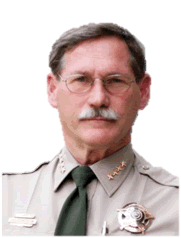
\includegraphics[height=0.28\textheight]{img/gil-gilbertson.png}
%            \\ Sheriff Gil Gilbertson \\ Josephine County \\
%            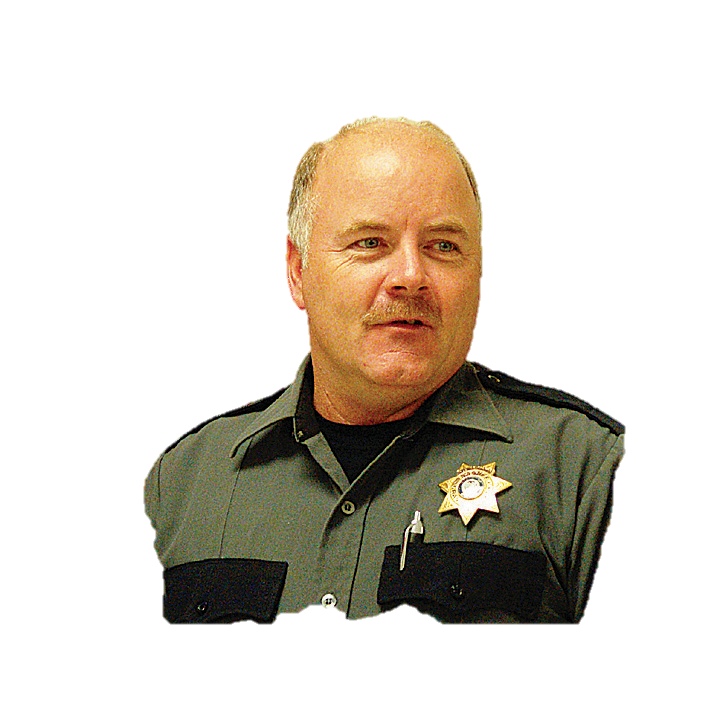
\includegraphics[height=0.28\textheight]{img/glenn-palmer.png}
%            \\ Sheriff Glenn Palmer \\ Grant County \\
%
%    \end{columns}
%\end{frame}
%
%\begin{frame}
%    \begin{columns}[onlytextwidth]
%        \column{0.5\textwidth}
%What bothered me the most regarding the conversation in Portland with the US
%Attorneys office was that they did not want to talk about the Constitution,
%but rather put all their confidence in the Supreme Court rulings. They even
%referred to the ``Supreme Law of the Land'' as the Supreme Court and were visibly
%upset that I would object to that notion
%        \column{0.5\textwidth}
%            \centering
%            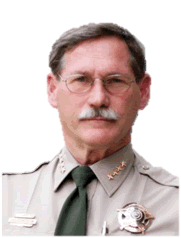
\includegraphics[width=0.75\textwidth]{img/gil-gilbertson.png}
%            \\ Sheriff Gil Gilbertson
%            \\ (Personal email, February 29, 2012)
%    \end{columns}
%\end{frame}
%
%\def\braces#1{[#1]}
%
%\begin{frame}{Summary and Opinion, January 13, 2012}
%    \begin{columns}[onlytextwidth]
%        \column{0.5\textwidth}
%            \centering
%            
\includegraphics[width=0.75\textwidth]{img/elmer-dickens.png}
%            \\ Attorney Elmer Dickens \\
%        \column{0.5\textwidth}
%\ldots it appears that the sheriff \braces{Gilbertson} does not believe that the US Supreme Court has the authority to interpret the meaning of the US Constitution\ldots
%    \end{columns}
%\end{frame}
%
%\begin{frame}{Summary and Opinion, January 13, 2012}
%    \begin{columns}[onlytextwidth]
%        \column{0.5\textwidth}
%        There are many Supreme Court cases going back over a hundred years\ldots \\
%        \vspace{16pt}
%        The federal Congress, well over one hundred years ago\ldots
%        \column{0.5\textwidth}
%            \centering
%            
\includegraphics[width=0.75\textwidth]{img/elmer-dickens.png}
%            \\ Attorney Elmer Dickens \\
%    \end{columns}
%\end{frame}
%
%\begin{frame}{Summary and Opinion, January 13, 2012}
%    \begin{columns}[onlytextwidth]
%        \column{0.5\textwidth}
%To put it bluntly, the opinion that federal agents do not have jurisdiction on federal property located within the State of Oregon is without support in the law and is meritless.
%        \column{0.5\textwidth}
%            \centering
%            
\includegraphics[width=0.75\textwidth]{img/elmer-dickens.png}
%            \\ Attorney Elmer Dickens \\
%    \end{columns}
%\end{frame}
%
%\begin{frame}{Supreme Court, 2012}
%    \centering
%    {\LARGE How \emph{trustworthy} are the decisions of the Supreme Court? } \\
%    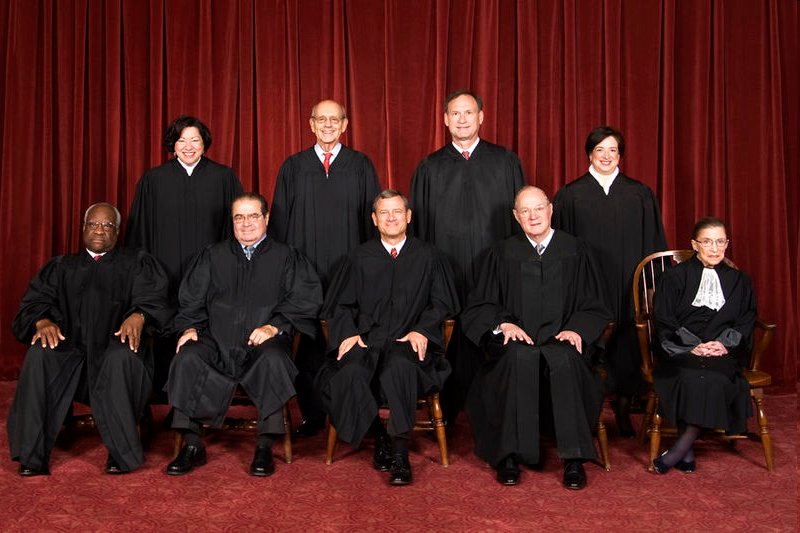
\includegraphics[width=0.9\textwidth]{img/supreme.png} \\
%\end{frame}
%
%\begin{frame}{Justice Clarence Thomas}
%    \begin{columns}[onlytextwidth]
%        \column{0.5\textwidth}
%            \centering
%            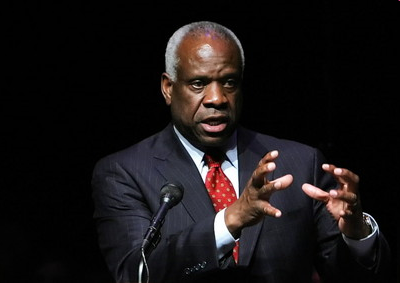
\includegraphics[width=0.75\textwidth]{img/clarence-thomas.png} \\
%        \column{0.5\textwidth}
%            There are really only two ways to interpret the Constitution: try to discern as best we can what the framers intended or \emph{make it up}.
%    \end{columns}
%\end{frame}
%
%\begin{frame}{Justice Clarence Thomas}
%    \begin{columns}[onlytextwidth]
%        \column{0.5\textwidth}
%            \centering
%            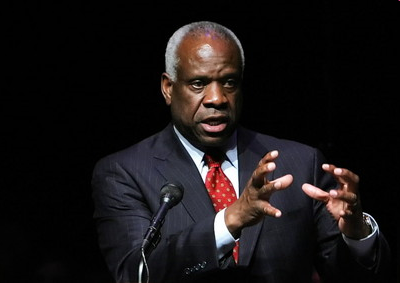
\includegraphics[width=0.75\textwidth]{img/clarence-thomas.png} \\
%        \column{0.5\textwidth}
%        Unless interpretive methodologies are tied to the
%        \textbf{\emph{original intent}} of the framers, they have no more basis
%        in the Constitution than the latest football scores. \\
%        \vspace{10pt}
%        Justice Clarence Thomas \\ Wall Street Journal Opinion \\ 20 October 2008
%    \end{columns}
%\end{frame}
%
%\begin{frame}
%    \centering
%    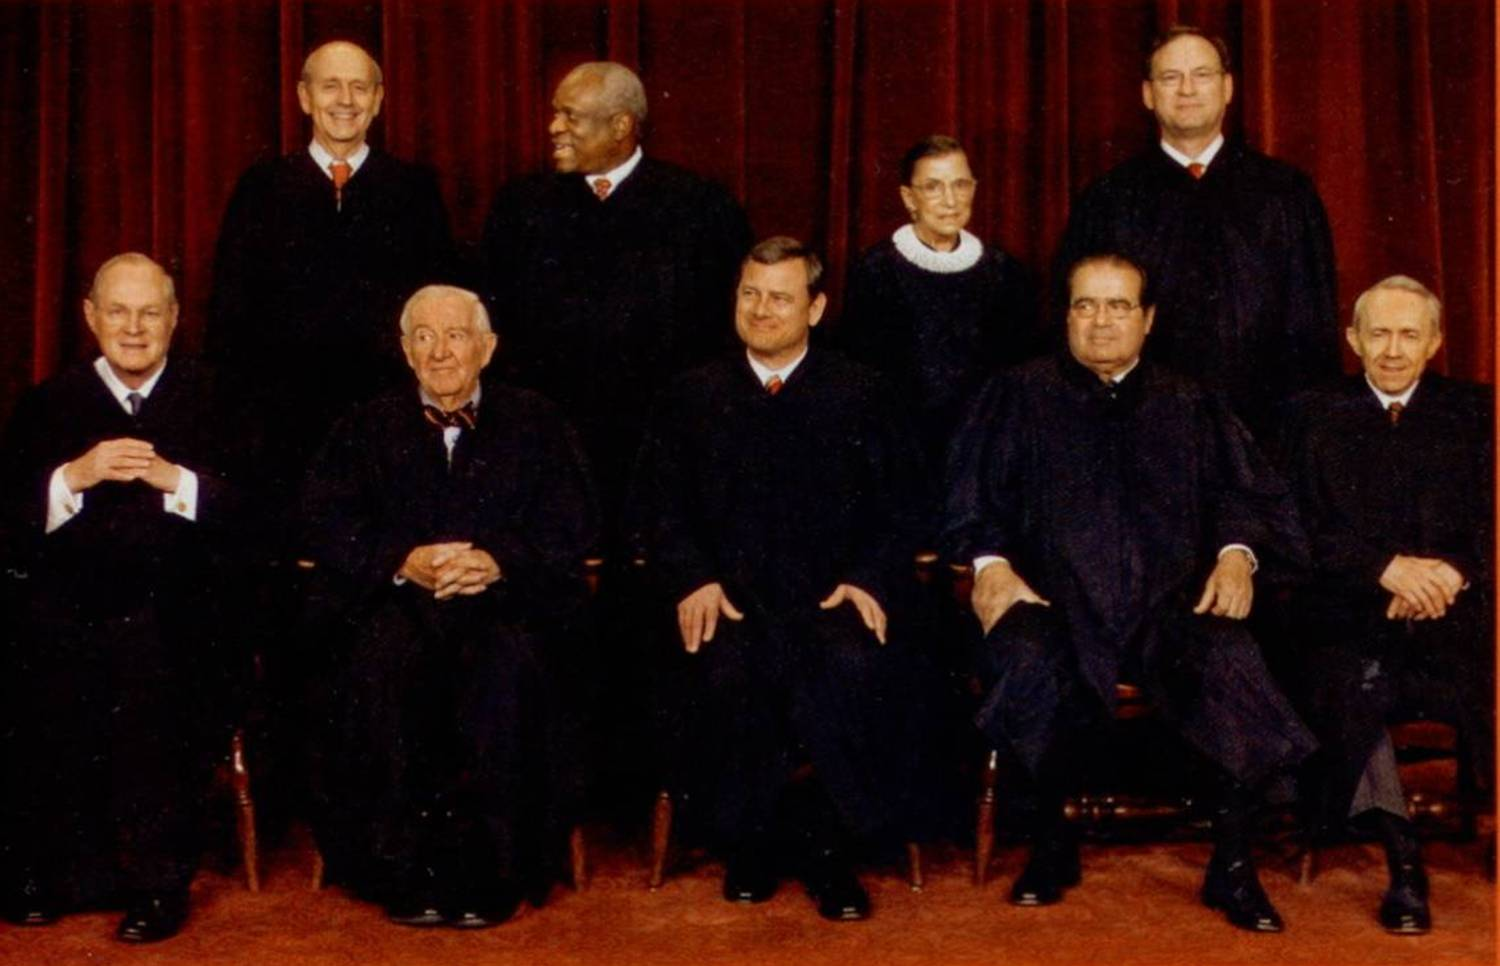
\includegraphics[width=0.95\textwidth]{img/thomas-breyer.jpg} \\
%    \pause
%    { \large \ldots they just make it up! } \\
%\end{frame}
%
%\begin{frame}
%    \begin{columns}[onlytextwidth]
%        \column{0.5\textwidth}
%            \centering
%            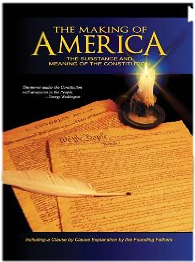
\includegraphics[width=0.75\textwidth]{img/making-of-america.png} \\
%            W. Cleon Skousen, Lawyer \\
%            1985, 888 pages \\
%
%        \column{0.5\textwidth}
%            ``\ldots \braces{the Supreme Court} began reversing previous decisions by the bushel basket.''
%    \end{columns}
%\end{frame}
%
%\begin{frame}{Usurpation --- Timothy B. Lewis}
%    Show a decent shot of Timothy B. Lewis and/or his book \\
%    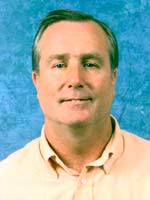
\includegraphics{img/timothy-lewis.png}
%\end{frame}
%
%\begin{frame}{The Supremacists --- Phyllis Schlafly}
%    \begin{columns}[onlytextwidth]
%        \column{0.5\textwidth}
%            \centering
%            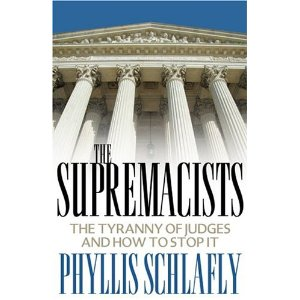
\includegraphics[width=0.75\textwidth]{img/the-supremacists.png} \\
%            2004, 246 pages \\
%
%        \column{0.5\textwidth}
%            \centering
%            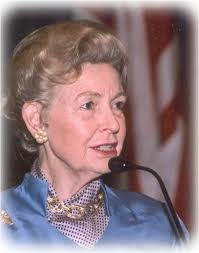
\includegraphics[width=0.75\textwidth]{img/phyllis-schlafly.png} \\
%            Lawyer \\
%    \end{columns}
%\end{frame}
%
%\begin{frame}{Men in Black}
%    \begin{columns}[onlytextwidth]
%        \column{0.5\textwidth}
%            \centering
%            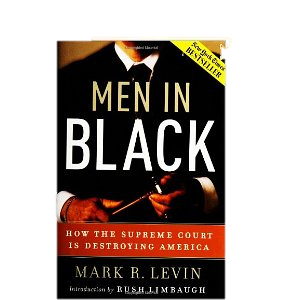
\includegraphics[width=0.75\textwidth]{img/men-in-black.png} \\
%
%        \column{0.5\textwidth}
%            \centering
%            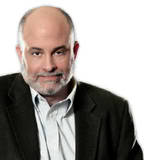
\includegraphics[width=0.75\textwidth]{img/mark-levin.png} \\
%            Mark Levin, Lawyer \\
%    \end{columns}
%\end{frame}
%
%%\begin{frame}{Betrayed by the Bench --- John A. Stormer}
%%    \begin{columns}[onlytextwidth]
%%        \column{0.5\textwidth}
%%            \centering
%%            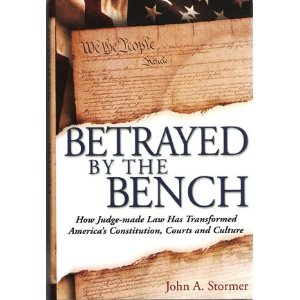
\includegraphics[width=0.75\textwidth]{img/betrayed-by-the-bench.png} \\
%%
%%        \column{0.5\textwidth}
%%            \centering
%%            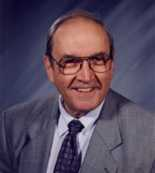
\includegraphics[width=0.75\textwidth]{img/john-stormer.png} \\
%%            John A. Stormer, \textbf{None Dare Call it Treason} \\
%%            \emph{(Millions of sales)} \\
%%    \end{columns}
%%\end{frame}
%
%%\begin{frame}{Constitutional Law for Enlighted Citizens --- Michael Farris}
%%    \begin{columns}[onlytextwidth]
%%        \column{0.5\textwidth}
%%            \centering
%%            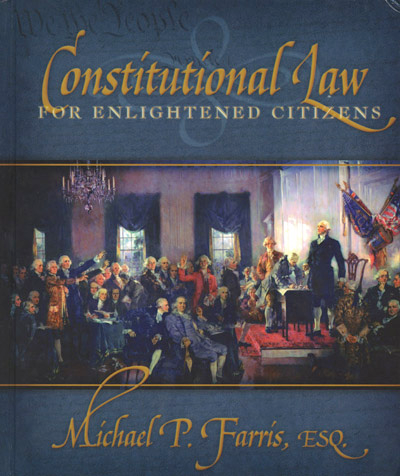
\includegraphics[width=0.75\textwidth]{img/constitutional-law.png} \\
%%            2006, 579 pages \\
%%
%%        \column{0.5\textwidth}
%%            \centering
%%            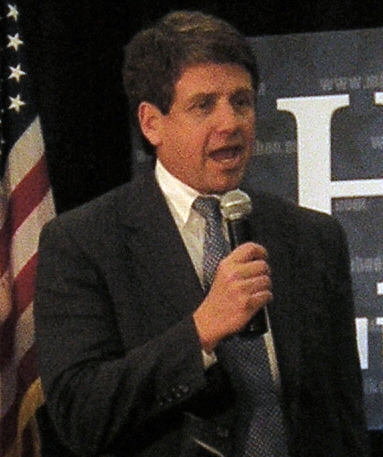
\includegraphics[width=0.75\textwidth]{img/michael-farris.png} \\
%%            Michael Farris, Lawyer
%%    \end{columns}
%%\end{frame}
%%
%%\begin{frame}{Constitutional Law for Enlighted Citizens --- Michael Farris}
%%    \begin{columns}[onlytextwidth]
%%        \column{0.5\textwidth}
%%            \centering
%%            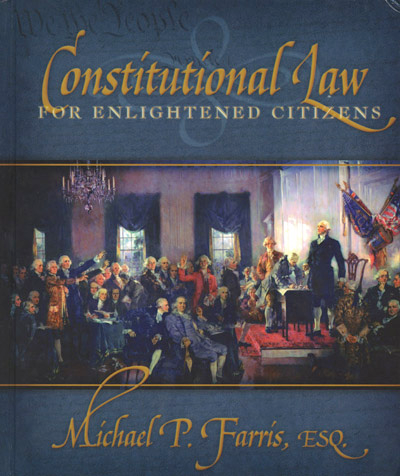
\includegraphics[width=0.75\textwidth]{img/constitutional-law.png} \\
%%            2006, 579 pages \\
%%
%%        \column{0.5\textwidth}
%%            ``The Court has twisted the Constitution and made it an instrument of tyranny\ldots  The Supreme Court makes law out of thin air.'' --- pages 4, 13
%%    \end{columns}
%%\end{frame}
%%
%%\begin{frame}{Constitutional Law for Enlighted Citizens --- Michael Farris}
%%    \begin{columns}[onlytextwidth]
%%        \column{0.5\textwidth}
%%            \centering
%%            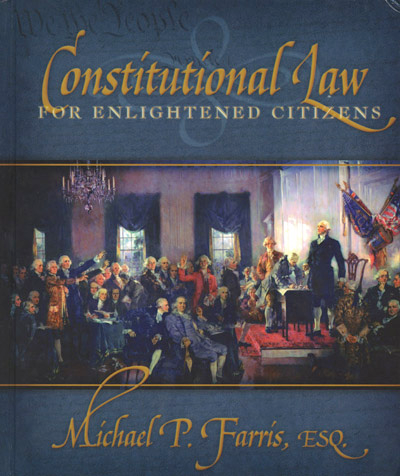
\includegraphics[width=0.75\textwidth]{img/constitutional-law.png} \\
%%            2006, 579 pages \\
%%
%%        \column{0.5\textwidth}
%%            ``All power to make laws shall be vested in Congress. \ldots Today, our freedoms are being stolen from us principally because we have allowed various agencies of government to violate this fundamental principle.'' --- page 8
%%    \end{columns}
%%\end{frame}
%
%\begin{frame}{U.S. Attorney S. Amanda Marshall}
%    \begin{columns}[onlytextwidth]
%        \column{0.5\textwidth}
%            \centering
%            
\includegraphics[width=0.75\textwidth]{img/amanda-marshall.png} \\
%            United States Attorney S. Amanda Marshall \\
%
%        \column{0.5\textwidth}
%            \centering
%            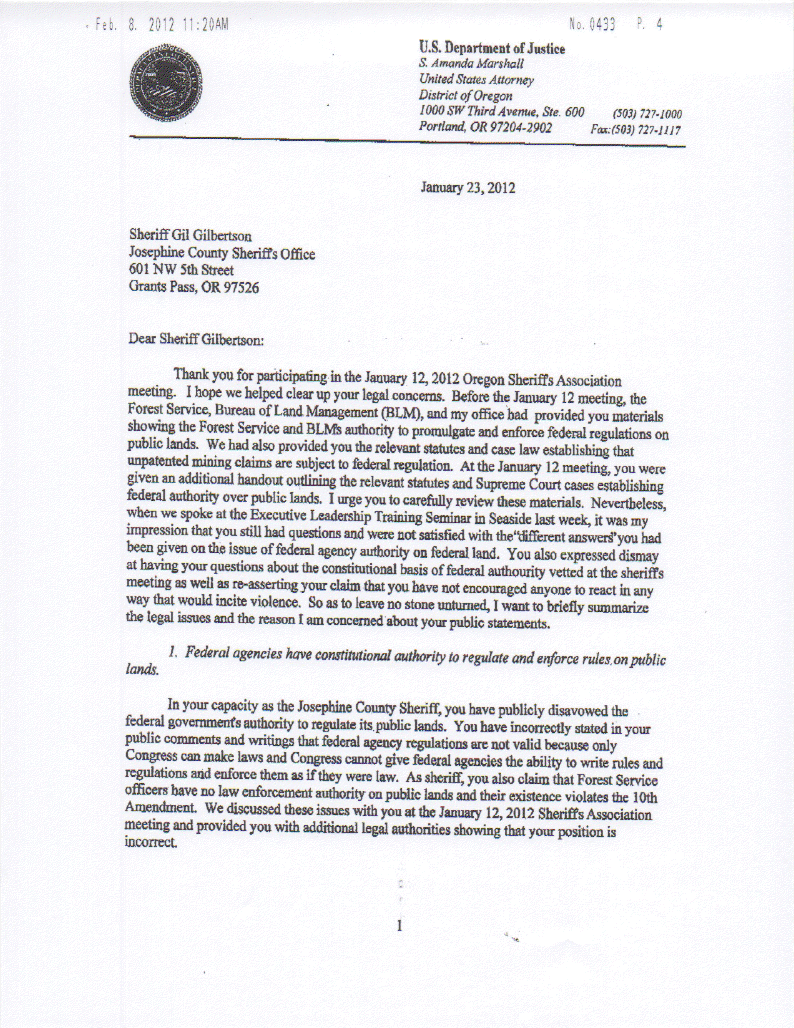
\includegraphics[width=0.75\textwidth]{img/marshall-letter.png} \\
%            January 23, 2012 \\
%    \end{columns}
%\end{frame}
%
%\begin{frame}{U.S. Attorney S. Amanda Marshall}
%    \begin{columns}[onlytextwidth]
%        \column{0.5\textwidth}
%            \centering
%            
\includegraphics[width=0.75\textwidth]{img/amanda-marshall.png} \\
%            United States Attorney S. Amanda Marshall \\
%
%        \column{0.5\textwidth}
%            ``Supreme Court precedent for the past one hundred years is clear: under the Property Clause, Congress may delegate rulemaking authority to its federal agencies\ldots''
%    \end{columns}
%\end{frame}
%
%\begin{frame}{The Supreme Court}
%    \centering
%    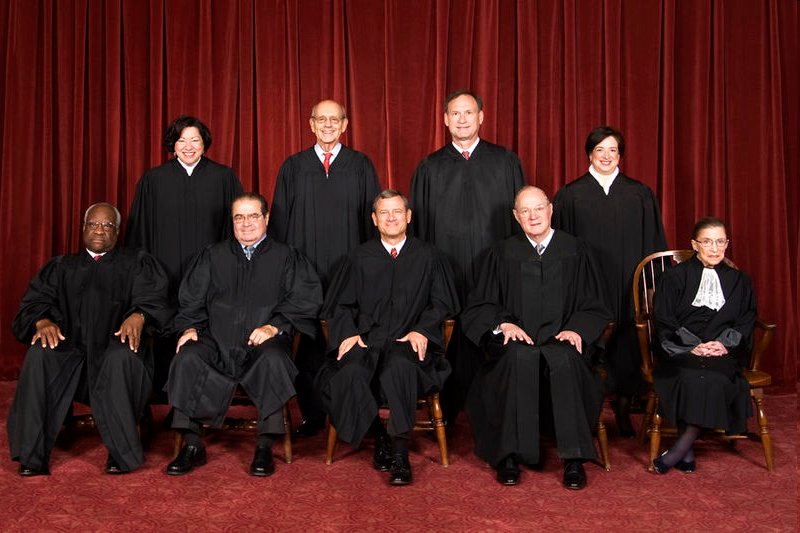
\includegraphics[width=0.75\textwidth]{img/supreme.png} \\
%    How trustworty is Supreme Court precendent? How trustworthy is their interpretation of ``the property clause''?
%\end{frame}
%
%\begin{frame}{U.S. Attorney S. Amanda Marshall}
%    \begin{columns}[onlytextwidth]
%        \column{0.5\textwidth}
%            \centering
%            
\includegraphics[width=0.75\textwidth]{img/amanda-marshall.png} \\
%            United States Attorney S. Amanda Marshall \\
%
%        \column{0.5\textwidth}
%            \centering
%            ``Your position is incorrect\ldots incorrect\ldots incorrect\ldots \\ erroneous\ldots \braces{You are on a} misguided crusade.'' \\
%            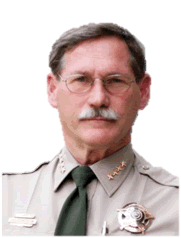
\includegraphics[width=0.3\textwidth]{img/gil-gilbertson.png} \\
%    \end{columns}
%\end{frame}
%
%\begin{frame}{U.S. Attorney S. Amanda Marshall}
%    \begin{columns}[onlytextwidth]
%        \column{0.5\textwidth}
%            \centering
%            
\includegraphics[width=0.75\textwidth]{img/amanda-marshall.png} \\
%            United States Attorney S. Amanda Marshall \\
%
%        \column{0.5\textwidth}
%            \centering
%            ``\braces{It is} your constitutional duty to promote respect for federal laws in your county, particularly when validated by the Supreme Court, whether you agree with them or not.'' \\
%            \vspace{10pt}
%            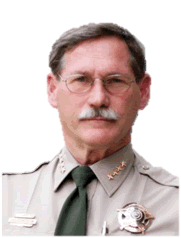
\includegraphics[width=0.3\textwidth]{img/gil-gilbertson.png} \\
%    \end{columns}
%\end{frame}
%
%\begin{frame}{The Oath?}
%    \centering
%    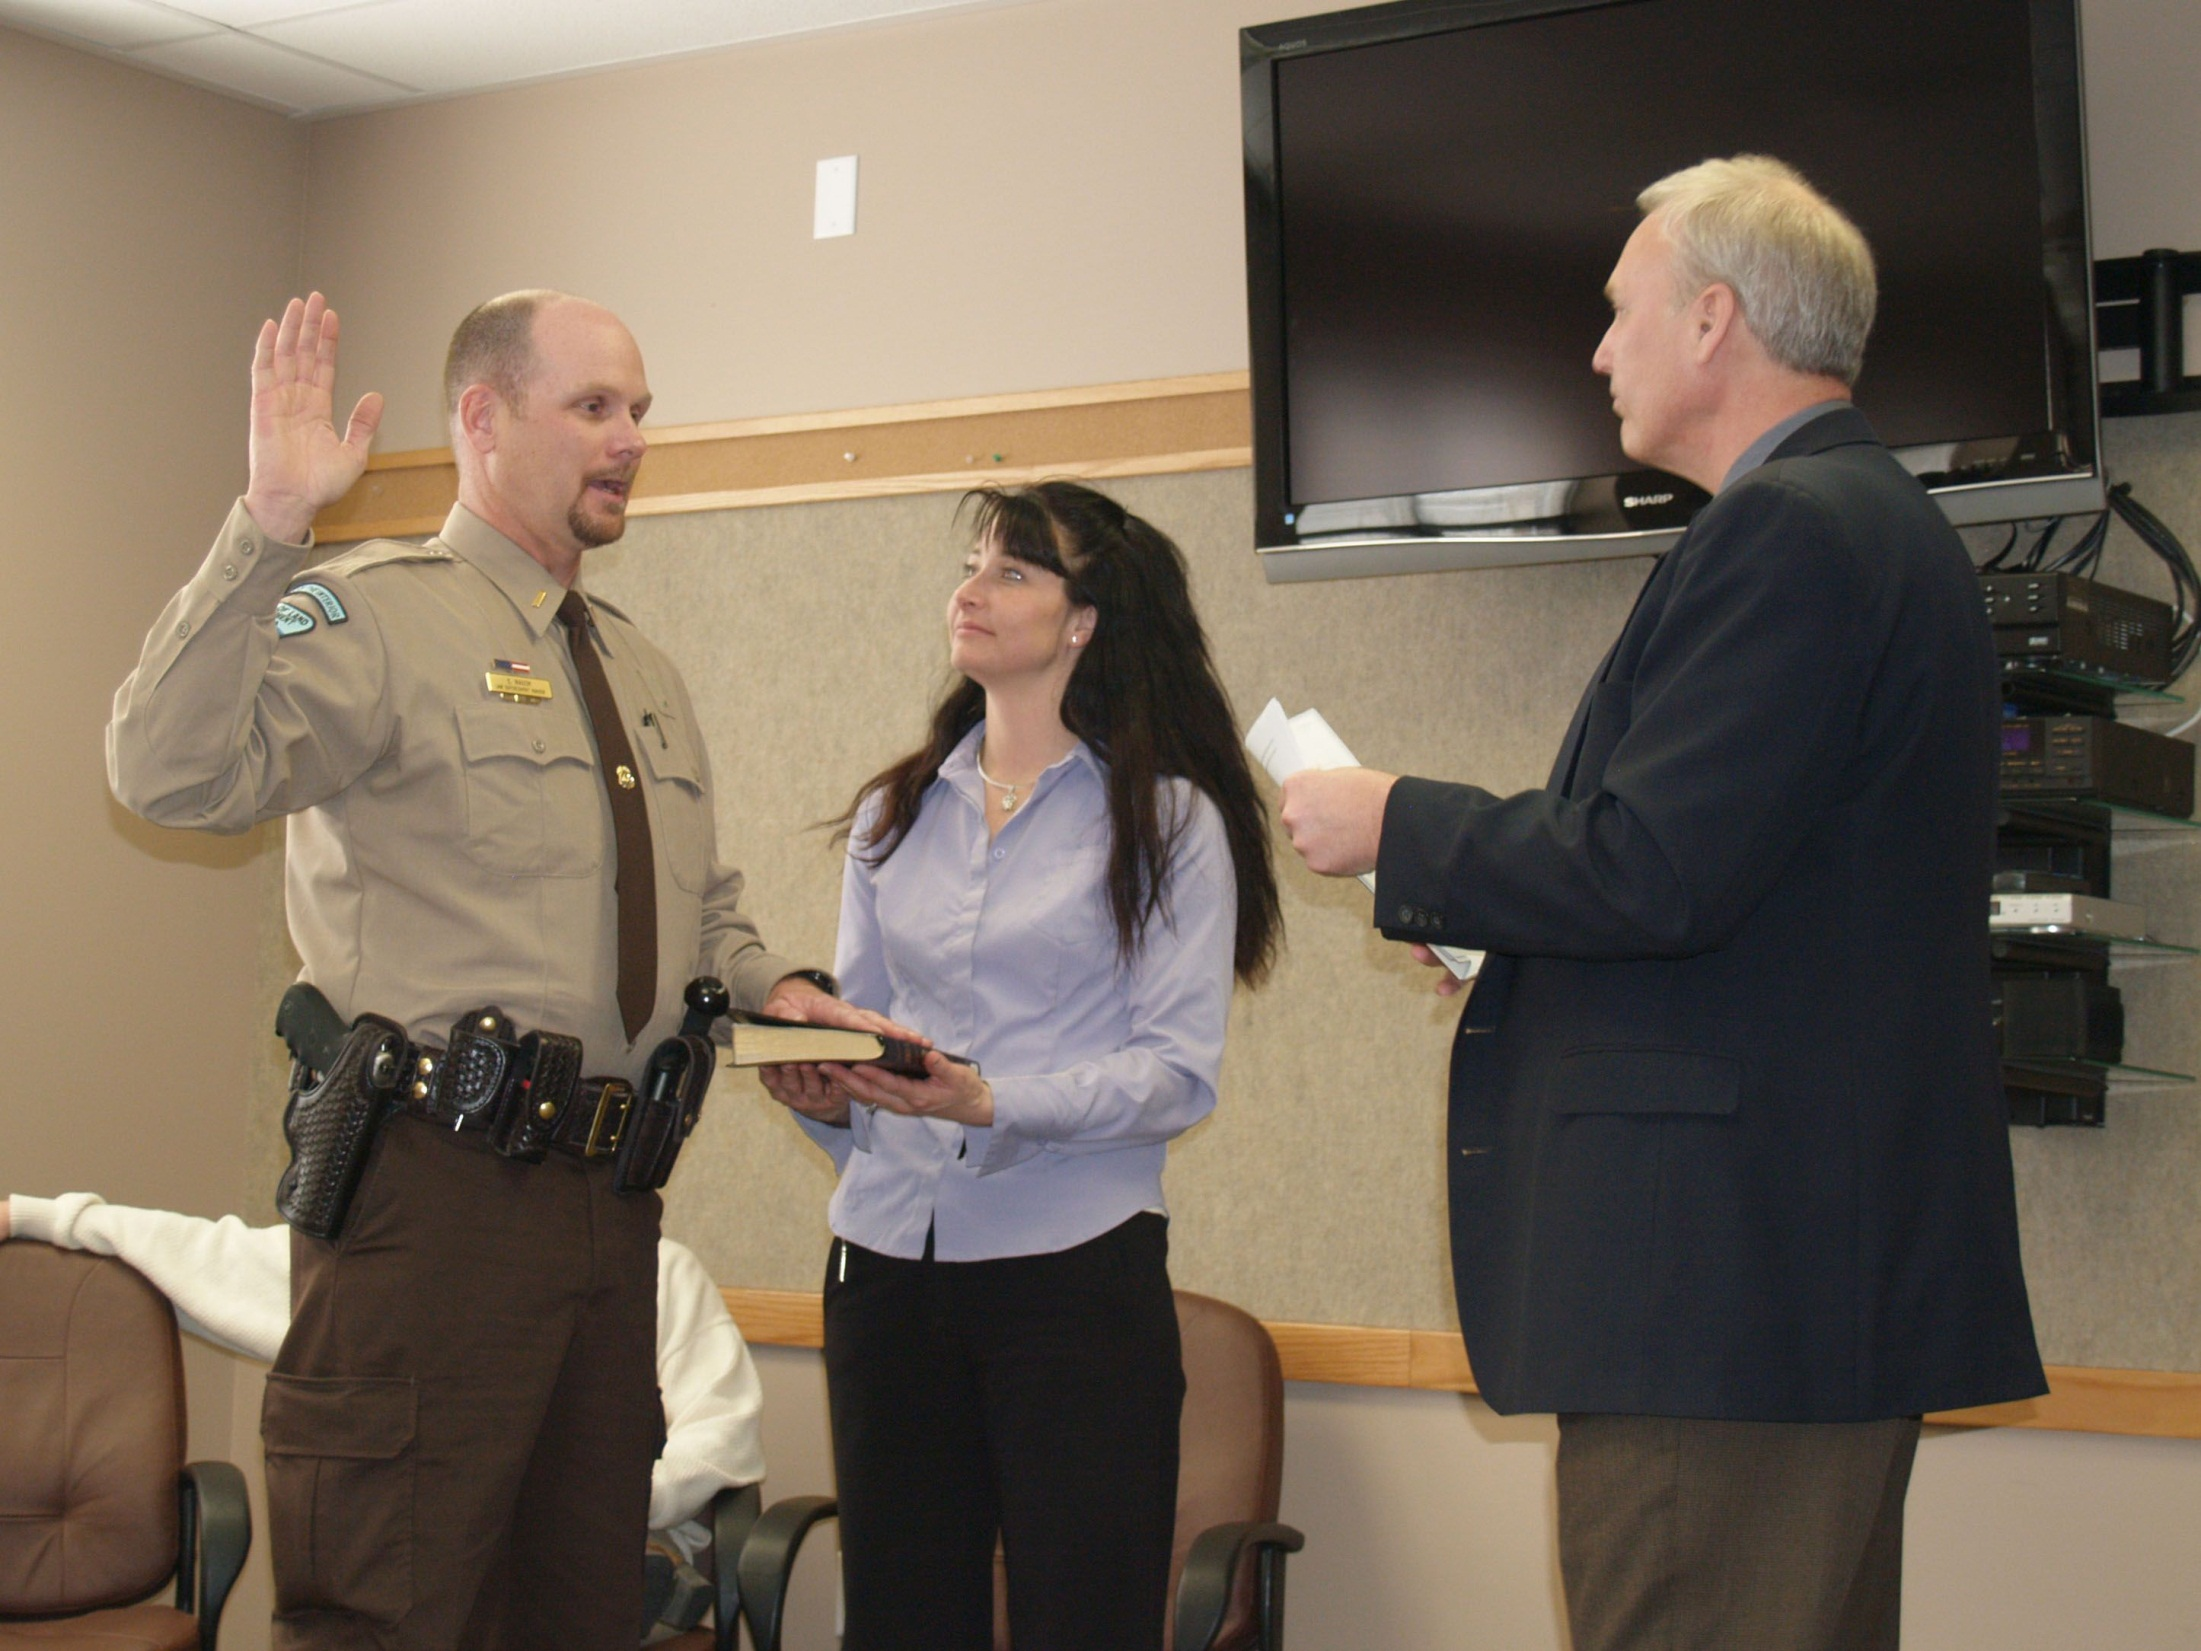
\includegraphics[width=0.7\textwidth]{img/oath.jpg} \\
%    I swear to uphold and defend the federal laws and regulations, particularly when validated by the Supreme Court, whether I agree with them or not!
%\end{frame}
%
%\begin{frame}{The Oath?}
%    \centering
%    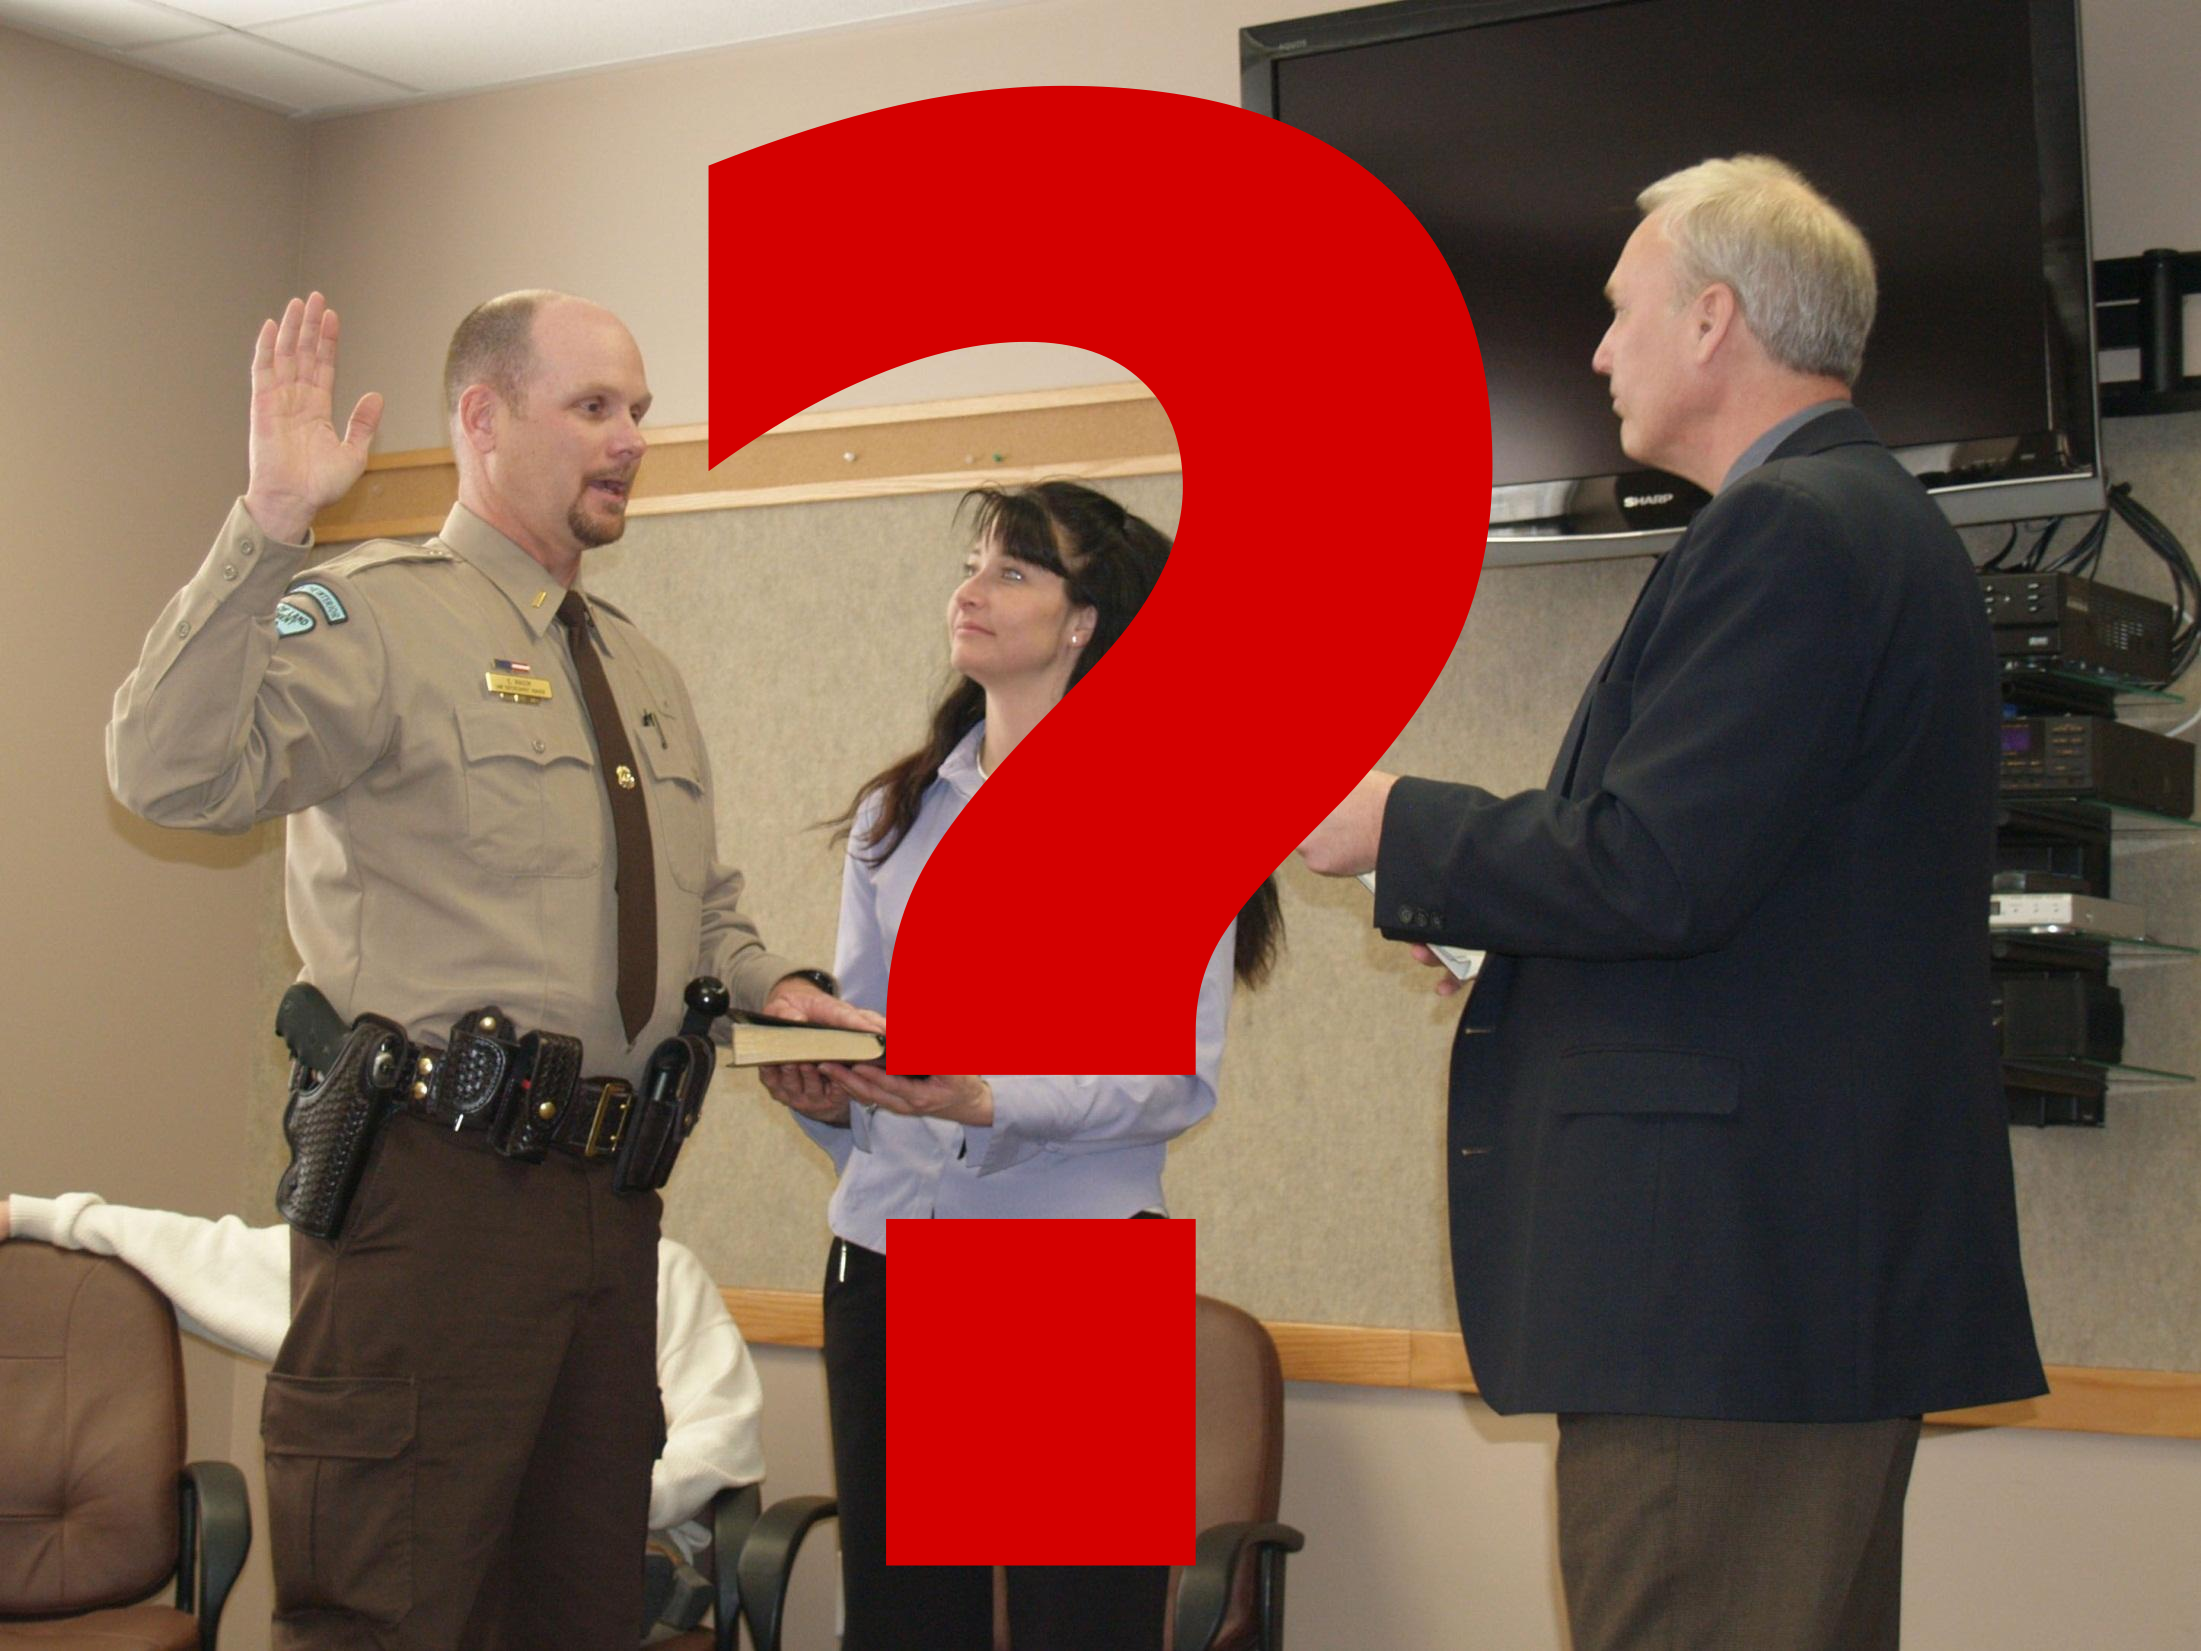
\includegraphics[width=0.7\textwidth]{img/oath-q.png} \\
%    I swear to uphold and defend the federal laws and regulations, particularly when validated by the Supreme Court, whether I agree with them or not!
%\end{frame}
%
%\begin{frame}{Duty-bound}
%    \centering
%    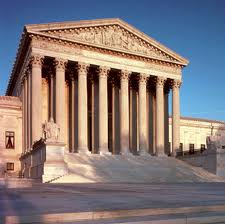
\includegraphics[width=0.3\textwidth]{img/court-bldg.png}
%    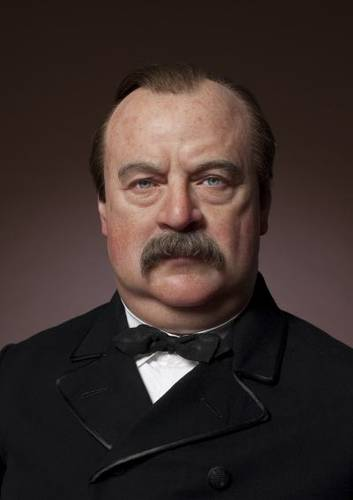
\includegraphics[width=0.3\textwidth]{img/cleveland.png}
%            % XXX Andy Griffith
%    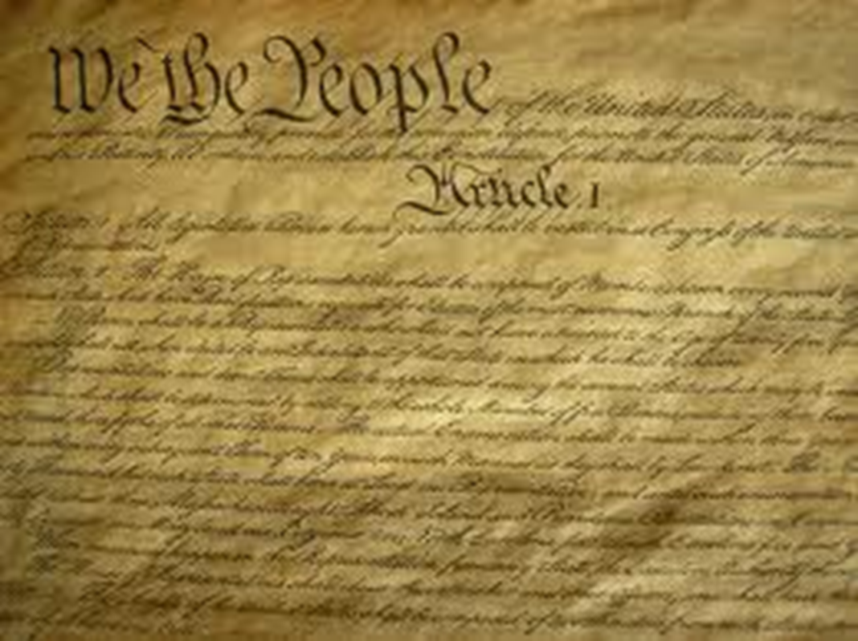
\includegraphics[width=0.3\textwidth]{img/constitution.png} \\
%    \vspace{18pt}
%    By oath, is a sheriff duty-bound to question the constitutionality of federal laws and court decisions? \\
%\end{frame}
%
%%\begin{frame}
%%    \begin{block}{Utah Oath of Office}
%%    I do solemnly swear (or affirm) that I will support, obey and defend the Constitution of the United States and the Constitution of this State, and that I will discharge the duties of my office with fidelity.
%%    \end{block}
%%\end{frame}
%%
%%\begin{frame}
%%    \begin{block}{Idaho Oath of Office}
%%    I do solemnly swear (or affirm, as the case may be) that I will support the Constitution of the United States, and the Constitution of the State of Idaho, and that I will faithfully discharge the duties of (insert office) according to the best of my ability.
%%    \end{block}
%%\end{frame}
%%
%%\begin{frame}
%%    \begin{block}{U.S. Senate Oath of Office}
%%    I do solemnly swear (or affirm) that I will support and defend the Constitution of the United States against all enemies, foreign and domestic; that I will bear true faith and allegiance to the same; that I take this obligation freely, without any mental reservation or purpose of evasion; and that I will well and faithfully discharge the duties of the office on which I am about to enter: So help me God.
%%    \end{block}
%%\end{frame}
%
%\begin{frame}{Sheriff Cleveland}
%    \begin{columns}[onlytextwidth]
%        \column{0.5\textwidth}
%            \centering
%            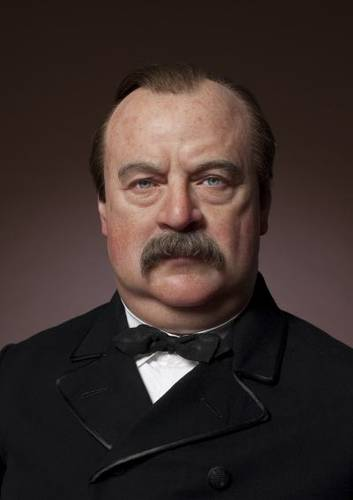
\includegraphics[width=0.75\textwidth]{img/cleveland.png} \\
%
%        \column{0.5\textwidth}
%            \centering
%            Sheriff Cleveland, 1871 \\
%            Erie County, New York
%    \end{columns}
%\end{frame}
%
%\begin{frame}{How Constitutional are ``Federal Laws''}
%    \begin{columns}[onlytextwidth]
%        \column{0.5\textwidth}
%            \centering
%            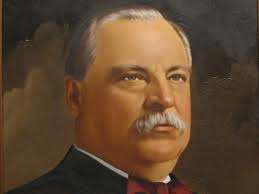
\includegraphics[width=0.75\textwidth]{img/cleveland2.png} \\
%
%        \column{0.5\textwidth}
%            Grover Cleveland was faithful to the Founder'’s Constitution and to
%            what he believed were God'’s commandments and common sense.  He
%            vetoed 584 Acts of Congress \\
%            \pause
%            \vspace{15pt}
%            ``I can find no warrant for such an appropriation in the Constitution.'' \\
%
%    \end{columns}
%\end{frame}
%
%\begin{frame}{How Constitutional are ``Federal Laws''}
%    \begin{columns}[onlytextwidth]
%        \column{0.5\textwidth}
%            \centering
%            \includegraphics[width=0.75\textwidth]{img/cleveland2.png} \\
%
%        \column{0.5\textwidth}
%            ``I ought to have a monument over me when I die, not for anything I have ever done, but for the foolishness I have put a stop to.''
%
%    \end{columns}
%\end{frame}
%
%\begin{frame}{How Constitutional are ``Federal Laws''}
%    \centering
%    { \Huge{The Freedom Index} } \\
%    \vspace{10pt}
%    \emph{A Congressional Scorecard Based on the U.S. Constitution} \\
%    \pause
%    January 9, 2012 \\
%    \vspace{15pt}
%    House / Senate Average Score on Ten Measures: \\
%    \vspace{20pt}
%    \pause
%    \color{red}{\Huge{44\%}} \\
%\end{frame}
%
%\begin{frame}{How Constitutional are ``Federal Laws''}
%    \centering
%    { \Large{United States Senate and House of Representatives }} \\
%    \vspace{20pt}
%    \includegraphics[width=0.75\textwidth]{img/house-senate-fail.png} \\
%\end{frame}
%
%\begin{frame}{Think Inside the Box}
%    \begin{columns}[onlytextwidth] \column{0.5\textwidth}
%            \centering
%            \includegraphics[width=0.75\textwidth]{img/box.png} \\
%
%        \column{0.5\textwidth}
%            \centering
%            \includegraphics[width=0.45\textwidth]{img/amanda-marshall.png} \\
%            \includegraphics[width=0.45\textwidth]{img/elmer-dickens.png} \\
%    \end{columns}
%\end{frame}
%
%\begin{frame}{Think Inside the Box}
%    \begin{columns}[onlytextwidth]
%        \column{0.5\textwidth}
%            \centering
%            \includegraphics[width=0.75\textwidth]{img/box.png} \\
%
%        \column{0.5\textwidth}
%            \begin{itemize}
%                \item Supreme Court decisions and acts of Congress ``over 100 years''
%                \pause
%                \item USC
%                \pause
%                \item Kleppe / FLPMA
%                \pause
%                \item Federal Register
%                \pause
%                \item Code of Federal Regulations
%            \end{itemize}
%    \end{columns}
%\end{frame}

\begin{frame}{Fundamental Principles}
    \begin{columns}[onlytextwidth]
        \column{0.5\textwidth}
            \centering
            \includegraphics[width=0.75\textwidth]{img/ben-franklin.png} \\
            Ben Franklin \\

        \column{0.5\textwidth}
            ``A frequent recurrence to \emph{fundamental principles}\ldots is absolutely necessary to preserve the blessings of liberty and keep a government free.''
    \end{columns}
\end{frame}

\begin{frame}{Fundamental Principles}
    \begin{columns}[onlytextwidth]
        \column{0.5\textwidth}
            \centering
            \includegraphics[width=0.75\textwidth]{img/patrick-henry.png} \\
            Patrick Henry \\

        \column{0.5\textwidth}
            ``No free government, or the blessing of liberty, can be preserved to any people but\ldots by a frequent recurrence to \emph{fundamental principles}.
    \end{columns}
\end{frame}

\begin{frame}{Fletcher vs. Peck, 10 U.S. 87}
    \centering
    \includegraphics[width=0.75\textwidth]{img/supreme-court-1810.png} \\
    Supreme Court, 1810 \\
\end{frame}

\begin{frame}{Fletcher vs. Peck, 10 U.S. 87}
    \begin{columns}[onlytextwidth]
        \column{0.5\textwidth}
            \centering
            \includegraphics[width=0.75\textwidth]{img/supreme-court-1810.png} \\
            Supreme Court, 1810 \\

        \column{0.5\textwidth}
            ``The security of a people against the misconduct of their rulers,
            must lie in the frequent recurrence to \emph{first principles}, and
            the imposition of adequate constitutional restrictions.''
    \end{columns}
\end{frame}

\begin{frame}
    \begin{columns}[onlytextwidth]
        \column{0.5\textwidth}
            ``The further back you can look, the farther forward you are likely to see.'' \\
            \vspace{20pt} Statehood, p. 19

        \column{0.5\textwidth}
            \centering
            \includegraphics[width=0.75\textwidth]{img/winston-churchill.png} \\
            Winston Churchill \\
    \end{columns}
\end{frame}

\begin{frame}{Two Contending Forces}
    \begin{columns}[onlytextwidth]
        \column{0.5\textwidth}
            \centering
            \includegraphics[height=0.75\textheight]{img/jefferson.png} \\
            Thomas Jefferson, 1824

        \column{0.5\textwidth}
            Men by their constitutions are naturally divided into two parties: \\
            \begin{enumerate}
                \item Those who fear and distrust the people, and wish to draw all powers from them into the hands of the higher classes.
                \item Those who identify themselves with the people, [and] have confidence in them.
            \end{enumerate}
    \end{columns}
\end{frame}

\begin{frame}{Roman Civil Law, 9 A. D.}
    \centering
    \includegraphics[width=0.75\textwidth]{img/europe-map.png} \\
    \only<1>{Roman Law \\}
%    \only<2>{Civil Law \\}
%    \only<3>{Roman Civil Law \\}
\end{frame}

\begin{frame}{Roman Law}
    \begin{columns}[onlytextwidth]
        \column{0.5\textwidth}
            \centering
            \includegraphics[height=0.55\textheight]{img/fasces-copy.jpg} \\
            Fasces \\

        \column{0.5\textwidth}
            \begin{itemize}
                \item All powerful central government
                \item National sovereignty
                \item Tax and control everything
                \item Watchdog everyone's business
                \item Promise prosperity and greatness
                \item Fight wars anywhere on earth
                \pause
                \item \emph{Do whatever is necessary. No exceptions. No limits\ldots}
            \end{itemize}
    \end{columns}
\end{frame}

\begin{frame}
    \centering
    \includegraphics[width=0.95\textwidth]{img/teutoburg.png} \\
    Battle of Teutoburg Forest, 9 A. D. \\
        Arminius of the Cherusci, Publius Quinctilius Varus \\
%    \only<2>{``We will rule our own territory!'' \\ }
\end{frame}

\begin{frame}
    \centering
    \includegraphics[width=0.95\textwidth]{img/teutoberg.jpg} \\
    Battle of Teutoburg Forest, 9 A. D. \\
        Arminius of the Cherusci, Publius Quinctilius Varus \\
%    \only<2>{``We will rule our own territory!'' \\ }
\end{frame}

\begin{frame}
    \centering
    \includegraphics[width=0.95\textwidth]{img/Varus01.jpg} \\
    Battle of Teutoburg Forest, 9 A. D. \\
        Arminius of the Cherusci, Publius Quinctilius Varus \\
%    \only<2>{``We will rule our own territory!'' \\ }
\end{frame}

\begin{frame}
    \centering
    \includegraphics[height=0.8\textheight]{img/teut2.jpg} \\
    Battle of Teutoburg Forest, 9 A. D. \\
        Arminius of the Cherusci, Publius Quinctilius Varus \\
%    \only<2>{``We will rule our own territory!'' \\ }
\end{frame}

\begin{frame}
    \centering
    \includegraphics[height=0.8\textheight]{img/teut3.jpg} \\
    Battle of Teutoburg Forest, 9 A. D. \\
        Arminius of the Cherusci, Publius Quinctilius Varus \\
%    \only<2>{``We will rule our own territory!'' \\ }
\end{frame}

\begin{frame}
    \centering
    \includegraphics[width=0.95\textwidth]{img/teut4.png} \\
    Battle of Teutoburg Forest, 9 A. D. \\
        Arminius of the Cherusci, Publius Quinctilius Varus \\
%    \only<2>{``We will rule our own territory!'' \\ }
\end{frame}

\begin{frame}
    \centering
    \includegraphics[width=0.95\textwidth]{img/teut5.png} \\
    Battle of Teutoburg Forest, 9 A. D. \\
        Arminius of the Cherusci, Publius Quinctilius Varus \\
%    \only<2>{``We will rule our own territory!'' \\ }
\end{frame}

\begin{frame}{Anglo-Saxon Common Law}
    \begin{columns}[onlytextwidth]
        \column{0.5\textwidth}
            Germanic brothers who entered England in 450 A. D., bringing with them Anglo-Saxon Common Law, the ``Guardian of Freedom''.

        \column{0.5\textwidth}
            \centering
            \includegraphics[height=0.55\textheight]{img/hengist-horsa.png} \\
            Hengist and Horsa \\
    \end{columns}
\end{frame}

%\begin{frame}{1215 A. D. --- Magna Carta}
%    \centering
%    Baronies force King John to sign the Magna Carta \\
%    \includegraphics[width=0.75\textwidth]{img/king-john.png} \\
%    ``\ldots to be sent to each of the English counties and to be read to all freemen.'' \\
%\end{frame}
%
%\begin{frame}{1215 A. D. --- Magna Carta}
%    \begin{columns}[onlytextwidth]
%        \column{0.5\textwidth}
%            \centering
%            \includegraphics[height=0.55\textheight]{img/magna-carta.png} \\
%
%        \column{0.5\textwidth}
%            ``All forests that have been created in our reign shall at once be disafforested.  River-banks that have been enclosed in our reign shall be treated similarly.'' \\
%            (Clause 47)  \\
%    \end{columns}
%\end{frame}
%
%\begin{frame}{1215 A. D. --- Magna Carta}
%    \begin{columns}[onlytextwidth]
%        \column{0.5\textwidth}
%            \centering
%            \includegraphics[height=0.55\textheight]{img/magna-carta.png} \\
%
%        \column{0.5\textwidth}
%            ``All evil customs relating to forest and warrens, foresters, warreners, sheriffs and their servants, or river-banks and their wardens, are at once to be investigated in every county  [and] are to be abolished completely and irrevocably.'' \\
%            (Clause 48)
%    \end{columns}
%\end{frame}

\begin{frame}{Germany, 1875 --- Hermanns Denkmal}
    \centering
    \includegraphics[width=0.75\textwidth]{img/hermans-denkmal.png} \\
\end{frame}

\begin{frame}{Germany, 1875 --- Hermanns Denkmal}
    \centering
    \includegraphics[width=0.75\textwidth]{img/herman2.png} \\
\end{frame}

\begin{frame}
    \begin{columns}[onlytextwidth]
        \column{0.5\textwidth}
            \centering
            \includegraphics[width=0.75\textwidth]{img/herman2.png} \\

        \column{0.5\textwidth}
            Arminius / Herman preserved ``Common Law''
            \pause
            \begin{itemize}
                \item Higher Law
                \pause
                \item Law of Nature
                \pause
                \item Constrast with Roman Law, based on coercion and force
            \end{itemize}
    \end{columns}
\end{frame}

\begin{frame}{Fundamental Principles of Common Law}
    \centering
    \includegraphics[width=0.75\textwidth]{img/schoolroom.png} \\
\end{frame}

\begin{frame}{Preserve Our Principles}
    \centering
    \includegraphics[width=0.75\textwidth]{img/herman3.png} \\
    Rome, go home! \\
\end{frame}

\begin{frame}{Preserve Our Principles}
    \begin{columns}[onlytextwidth]
        \column{0.5\textwidth}
            \centering
            \includegraphics[width=0.75\textwidth]{img/jefferson.png} \\
            Thomas Jefferson \\

        \column{0.5\textwidth}
            Restore the Ancient Principles\ldots
            \begin{itemize}
                \item \ldots of Common Law
                \item \ldots of the Old Testament
            \end{itemize}
    \end{columns}
\end{frame}

\begin{frame}{Government of Ancient Israel}
    \centering
    \includegraphics[width=0.75\textwidth]{img/moses.jpg} \\
    \only<1>{
        And Moses' father-in-law said unto him: Thou shalt teach them ordinances and laws, and shalt show them the way wherein they must walk and the work that they must do.
    }
    \only<2>{ Groups of tens, fifties, hundreds, thousands, to successfully govern three million people \\ }
%    \only<3>{ This became the basis of ``Common'', or ``People's'' Law \\ }
\end{frame}

\begin{frame}{Preserve Our Principles}
    \begin{columns}[onlytextwidth]
        \column{0.5\textwidth}
            \centering
            \includegraphics[width=0.75\textwidth]{img/moses.jpg} \\
            Anglo-Saxon Common Law \color{red}\\

        \column{0.5\textwidth}
            \begin{itemize}
                \item Ten families --- a ``Tithing'', led by a ``tithing man''
                \item Two tithings --- a ``Vil'', led by a ``vil man''
                \item Two vils --- a ``Hundred'', led by a ``hundred man''
                \item Several hundreds --- a ``Shire'', led by a ``shire reef''
            \end{itemize}
    \end{columns}
\end{frame}

\begin{frame}{Roman Law v. Common Law}
    \begin{columns}[onlytextwidth]
        \column{0.5\textwidth}
            \centering
            \includegraphics[height=0.75\textheight]{img/fasces-copy.jpg} \\

        \column{0.5\textwidth}
            \centering
            \includegraphics[height=0.35\textheight]{img/hh-coin.png} \\
            \includegraphics[height=0.35\textheight]{img/israel-coin.png} \\
    \end{columns}
\end{frame}

%\begin{frame}{``Shire Reef'' $\rightarrow$ ``Sheriff''}
%    \centering
%    \includegraphics[width=.9\textwidth]{img/shire-reef.png} \\
%\end{frame}
%
%\unitlength=1in
%\begin{frame}
%    \centering
%    \includegraphics[width=.9\textwidth]{img/sheriffs.png} \\
%    \pause
%    \Put(0.3,6){\textbf{\color{blue}{\Large{Maryland, 1634}}}}
%    \pause
%    \Put(3,0.8){\textbf{\color{blue}{\Large{Virginia, 1651}}}}
%\end{frame}
%
%\begin{frame}{Utah Territorial Act, September 9, 1850}
%    \centering
%    \begin{block}{}
%        ``\ldots and the same is hereby, created into a \emph{temporary government}, by the name of the Territory of Utah\ldots''
%    \end{block}
%    \vspace{10pt}
%    \includegraphics[width=0.75\textwidth]{img/utah-terr.png} \\
%\end{frame}
%
%\begin{frame}{Utah Territory, 1894}
%    \begin{columns}[onlytextwidth]
%        \column{0.5\textwidth}
%            \centering
%            \includegraphics[height=0.75\textheight]{img/utah-state.png} \\
%
%        \column{0.5\textwidth}
%            \Huge{People \\ + Territory \\ + Governance \\ = State}
%    \end{columns}
%\end{frame}
%
%\begin{frame}{Utah Territory, 1894}
%    \begin{columns}[onlytextwidth]
%        \column{0.5\textwidth}
%            \centering
%            \includegraphics[height=0.75\textheight]{img/utah-state.png} \\
%
%        \column{0.5\textwidth}
%            \begin{block}{Utah Enabling Act \textbf{Compact}, July 16, 1894}
%                As of May 3, 2012, it appears there are still \textbf{\emph{{\color{red}seven violations}}} of the Compact on the part of the Federal Government.
%            \end{block}
%    \end{columns}
%\end{frame}
%
%\begin{frame}{Utah Territory}
%    \begin{columns}[onlytextwidth]
%        \column{0.5\textwidth}
%            \centering
%            \includegraphics[height=0.75\textheight]{img/constitution.png} \\
%
%        \column{0.5\textwidth}
%            \begin{block}{Admissions Clause}
%                ``New States may be admitted by Congress into this Union\ldots''
%            \end{block}
%    \end{columns}
%\end{frame}
%
%\begin{frame}{Utah, January 4, 1896}
%    \centering
%    \includegraphics[height=0.75\textheight]{img/utah-constitution.png} \\
%\end{frame}
%
%\unitlength=1pt
%\begin{frame}{Jurisdiction Clause Family}
%    \centering
%    \includegraphics[height=0.85\textheight]{img/family.png} \\
%    \huge{\textbf{ \color{white}
%        \pause
%        \Put(25, 300){\begin{sideways}\colorbox{blue}{Admissions}\end{sideways}}
%        \pause
%        \Put(60, 300){\begin{sideways}\colorbox{blue}{Claims}\end{sideways}}
%        \pause
%        \Put(90, 300){\begin{sideways}\colorbox{blue}{Property}\end{sideways}}
%        \pause
%        \Put(134, 300){\begin{sideways}\colorbox{blue}{Guarantee}\end{sideways}}
%        \pause
%        \Put(168, 300){\begin{sideways}\colorbox{blue}{Enclave}\end{sideways}}
%        \pause
%        \Put(200, 300){\begin{sideways}\colorbox{blue}{Engagements}\end{sideways}}
%        \pause
%        \Put(235, 300){\begin{sideways}\colorbox{blue}{Supremacy}\end{sideways}}
%    }}
%\end{frame}
%
%\begin{frame}
%    \begin{varblock}[0.8\textwidth]{Truism}
%        \Large{We may only delegate to government that which we have the right to do ourselves.}
%    \end{varblock}
%\end{frame}
%
%\begin{frame}{State of Utah}
%    \begin{columns}[onlytextwidth]
%        \column{0.5\textwidth}
%            \centering
%            \includegraphics[height=0.75\textheight]{img/utah-constitution.png} \\
%
%        \column{0.5\textwidth}
%            The new state legislature began passing laws to protect life, liberty, and property. \\
%            \vspace{20pt}
%            County Sheriff established by:
%            \begin{itemize}
%                \item 17-16-1
%                \item 17-22-1.5
%                \item 20A-9-201
%                \item 53-6-202(4)
%                \item 53-6-205
%            \end{itemize}
%    \end{columns}
%\end{frame}
%
%\begin{frame}
%    \begin{varblock}[0.8\textwidth]{Definition}
%        A legal dictionary defines the Sheriff as ``\ldots a creature of law created by the \textbf{sovereign power in the state}\ldots'' 
%    \end{varblock}
%\end{frame}
%
%\begin{frame}{Mack / Printz v. The United States of America, 1997}
%    \centering
%    \includegraphics[width=0.65\textwidth]{img/printz-mack.jpg} \\
%\end{frame}
%
%\begin{frame}{Mack / Printz v. The United States of America, 1997}
%    \begin{columns}[onlytextwidth]
%        \column{0.5\textwidth}
%            \centering
%            \includegraphics[height=0.75\textheight]{img/scalia.jpg} \\
%            Justice Antonin Scalia \\
%
%        \column{0.5\textwidth}
%            \begin{block}{Mack/Printz v. USA}
%                ``\ldots it is incontestible that the Constitution established a system of `dual sovereignty'.''
%            \end{block}
%            \pause
%            {
%                \color{red}
%                \emph{Did the United States Constitution establish a system of ``dual sovereignty''?}
%            }
%    \end{columns}
%\end{frame}
%
%\begin{frame}{Mack / Printz v. The United States of America, 1997}
%    \begin{columns}[onlytextwidth]
%        \column{0.5\textwidth}
%            \centering
%            \includegraphics[height=0.75\textheight]{img/scalia.jpg} \\
%            Justice Antonin Scalia \\
%
%        \column{0.5\textwidth}
%            \begin{block}{Mack/Printz v. USA}
%                ``Although the States surrendered many of their powers to the new Federal Government\ldots''
%            \end{block}
%            \pause
%            {
%                \color{red}
%                \emph{Did the States ``[surrender] many of their powers to the new Federal Government''?}
%            }
%    \end{columns}
%\end{frame}
%
%\begin{frame}{Tea Party}
%    \centering
%    \includegraphics[width=0.75\textwidth]{img/tea-party.jpg} \\
%    \begin{block}{}Current choices in Washington D. C. are ``a grave threat to our national sovereignty.'' \end{block}
%    \begin{itemize}
%        \item What is national sovereignty?
%        \item Did the United States Constitution establish national sovereignty?
%        \item What is state sovereignty?
%    \end{itemize}
%\end{frame}
%
%\begin{frame}{Alexander Hamilton, Constitutional Convention}
%    \begin{columns}[onlytextwidth]
%        \column{0.5\textwidth}
%            \centering
%            \includegraphics[height=0.75\textheight]{img/hamilton.png} \\
%            Alexander Hamilton \\
%
%        \column{0.5\textwidth}
%            \begin{block}{}
%                ``Two sovereignties cannot co-exist within the same limits.''
%            \end{block}
%            \pause
%            \vspace{15pt}
%            In other words, \emph{state sovereignty} and \emph{national sovereignty} cannot exist at the same time.
%    \end{columns}
%\end{frame}
%
%\begin{frame}{Alexander Hamilton, Constitutional Convention}
%    \begin{columns}[onlytextwidth]
%        \column{0.5\textwidth}
%            \centering
%            \includegraphics[height=0.75\textheight]{img/hamilton.png} \\
%            Alexander Hamilton \\
%
%        \column{0.5\textwidth}
%            \begin{block}{}
%                ``[We must establish] a complete sovereignty in the General Government\ldots The general power, if it preserves itself, must swallow up the state powers.''
%            \end{block}
%            \pause
%            {
%                \centering
%                \includegraphics[width=0.5\textwidth]{img/red-light.png} \\
%            }
%    \end{columns}
%\end{frame}
%
%\begin{frame}{Thomas Jefferson, 1824}
%    \begin{columns}[onlytextwidth]
%        \column{0.5\textwidth}
%            \centering
%            \includegraphics[height=0.75\textheight]{img/jefferson.png} \\
%
%        \column{0.5\textwidth}
%            ``In every country these two parties exist.''
%    \end{columns}
%\end{frame}
%
%\begin{frame}{Two Contending Forces}
%    \begin{columns}[onlytextwidth]
%        \column{0.5\textwidth}
%            \begin{varblock}[0.9\textwidth]{}\huge{We the people of the United States is a nationalist system}\end{varblock}
%
%        \column{0.5\textwidth}
%            \begin{varblock}[0.9\textwidth]{}\huge{We the people of the States of NH, MA, RI, NY, PA, NJ, \ldots  are a federative system.}\end{varblock}
%    \end{columns}
%    \textbf{\huge{ \color{red}
%        \Put(155,150){v.}
%    }}
%\end{frame}
%
%\begin{frame}{Nationalists}
%\begin{table}[h]
%\centering
%\begin{tabular}{lcccccc} 
%    \includegraphics[width=0.75\textwidth,height=.3\textheight,keepaspectratio=true]{img/hamilton-portrait.png} &
%    \includegraphics[width=0.75\textwidth,height=.3\textheight,keepaspectratio=true]{img/story-portrait.png} &
%    \includegraphics[width=0.75\textwidth,height=.3\textheight,keepaspectratio=true]{img/morris-portrait.png} \\
%    Alexander Hamilton & 
%    Joseph Story &
%    Gouvernor Morris \\
%    \includegraphics[width=0.75\textwidth,height=.3\textheight,keepaspectratio=true]{img/lincoln-portrait.png} &
%    \includegraphics[width=0.75\textwidth,height=.3\textheight,keepaspectratio=true]{img/marshall-portrait.png} &
%    \includegraphics[width=0.75\textwidth,height=.3\textheight,keepaspectratio=true]{img/daniel-webster-portrait.png} \\
%    Abraham Lincoln &
%    John Marshall &
%    Daniel Webster &
%\end{tabular}
%\end{table}
%\end{frame}
%
%\begin{frame}{Remember\ldots}
%    \begin{columns}[onlytextwidth]
%        \column{0.5\textwidth}
%            \centering
%            \huge{ROMAN LAW} \\
%            \vspace{20pt}
%            \includegraphics[height=0.55\textheight]{img/fasces-copy.jpg} \\
%
%        \column{0.5\textwidth}
%            \begin{itemize}
%                \item All powerful central government
%                \item National sovereignty
%                \item Tax and control everything
%                \item Watchdog everyone's business
%                \item Promise prosperity and greatness
%                \item Fight wars anywhere on earth
%            \end{itemize}
%    \end{columns}
%\end{frame}
%
%\begin{frame}
%    \begin{columns}[onlytextwidth]
%        \column{0.5\textwidth}
%            \centering
%            \includegraphics[width=0.75\textwidth]{img/andrew-johnson.jpg} \\
%            Andrew Johnson \\
%
%        \column{0.5\textwidth}
%            \begin{block}{News Release, August 14, 1866}
%                The National Union Party declares ``the absolute supremacy of the National Government''
%            \end{block}
%    \end{columns}
%\end{frame}

\begin{frame}{1914}
    \centering
    \includegraphics[width=.9\textwidth]{img/lincoln-memorial.jpg} \\
\end{frame}

\begin{frame}
    \begin{columns}[onlytextwidth]
        \column{0.5\textwidth}
            \centering
            \includegraphics[width=0.75\textwidth]{img/americas-caesar.png} \\

        \column{0.5\textwidth}
            \begin{block}{America's Caesar}
                The Decline and Fall of Republican Government in the United States of America
            \end{block}
    \end{columns}
\end{frame}

\begin{frame}
    \begin{columns}[onlytextwidth]
        \column{0.5\textwidth}
            \centering
            \includegraphics[width=0.75\textwidth]{img/dime-usa-fasces-2.jpg} \\
            1916 - 1945 \\

        \column{0.5\textwidth}
            \centering
            \includegraphics[height=0.55\textheight]{img/fasces-copy.jpg} \\
            Roman Law\\

    \end{columns}
\end{frame}

\begin{frame}
    \centering
    \includegraphics[width=.9\textwidth]{img/obama-fasces.jpg} \\
\end{frame}

\begin{frame}
    \centering
    \includegraphics[height=.8\textheight]{img/fasces/badge_description.jpg} \\
    Los Angeles Police Dept. badge, developed 1939 - 1941 \\
\end{frame}
\begin{frame}
    \centering
    \includegraphics[height=.8\textheight]{img/fasces/coin.jpg} \\
    Italian East Africa Campaign medal, 1936 \\
\end{frame}
\begin{frame}
    \centering
    \includegraphics[width=.9\textwidth]{img/fasces/fake-fasces.jpg} \\
    Catalonia (largely autonomous Spanish province), 2006 \\
\end{frame}
\begin{frame}
    \centering
    \includegraphics[height=.8\textheight]{img/fasces/fasces13.jpg} \\
    Adopted 1877. Text reads ``Union and Consitution''. Colorado's state website claims ``The Roman fasces is the insignia of a republican form of government\ldots The axe symbolizes authority and leadership.'' \\
\end{frame}
\begin{frame}
    \centering
    \includegraphics[height=.8\textheight]{img/fasces/fasces5coin.jpg} \\
\end{frame}
\begin{frame}
    \centering
    \includegraphics[width=.9\textwidth]{img/fasces/fasces_congress.jpg} \\
\end{frame}
%\begin{frame}
%    \centering
%    \includegraphics[width=.9\textwidth]{img/fasces/Fasces_Mussolini-Hitler_mark.jpg} \\
%\end{frame}
\begin{frame}
    \centering
    \includegraphics[width=.9\textwidth]{img/fasces/fasces-stuff.jpg} \\
    Statue by John Quincy Adams Ward, 1882.
\end{frame}
\begin{frame}
    \centering
    \includegraphics[width=.9\textwidth]{img/fasces/ows.jpg} \\
    Federal Hall, New York City \\
\end{frame}
\begin{frame}
    \centering
    \includegraphics[height=.8\textheight]{img/fasces/flag-fasces.jpg} \\
\end{frame}
\begin{frame}
    \centering
    \includegraphics[height=.8\textheight]{img/fasces/french-republic-symbol.png} \\
    National Symbol of France, adopted 1953. This symbol is used to represent France in the U.N. Assembly building. \\
\end{frame}
\begin{frame}
    \centering
    \includegraphics[height=.8\textheight]{img/fasces/houdon-front.jpg} \\
    Statue by Jean-Antoine Houdon, completed 1791. Commissioned by Virgina's legislature, and on display at Colonial Williamsburg. \\
\end{frame}
\begin{frame}
    \centering
    \includegraphics[height=.8\textheight]{img/fasces/italy-fasces-coin.jpg} \\
    Italian 5 lira piece, 1928 \\
\end{frame}
\begin{frame}
    \centering
    \includegraphics[height=.9\textheight]{img/fasces/jfk.jpg} \\
\end{frame}
\begin{frame}
    \centering
    \includegraphics[width=.9\textwidth]{img/fasces/lincoln_fasces.jpg} \\
\end{frame}
\begin{frame}
    \centering
    \includegraphics[width=.9\textwidth]{img/fasces/manhole.JPG} \\
\end{frame}
\begin{frame}
    \centering
    \includegraphics[height=.8\textheight]{img/fasces/mp.jpg} \\
\end{frame}
\begin{frame}
    \centering
    \includegraphics[height=.8\textheight]{img/fasces/tax-court.png} \\
    The Tax Court took on its present form in 1969 \\
\end{frame}
\begin{frame}
    \centering
    \includegraphics[height=.8\textheight]{img/fasces/teut1.jpg} \\
    Detail of frieze in the U.S. Capitol rotunda. The frieze was designed in 1859 and begun in 1877, but wasn't fully complete until 1953. \\
\end{frame}
\begin{frame}
    \centering
    \includegraphics[width=.9\textwidth]{img/fasces/tunnel.jpg} \\
\end{frame}
\begin{frame}
    \centering
    \includegraphics[height=.8\textheight]{img/fasces/washington1.jpg} \\
    By Horatio Greenough, completed in 1840, and now found in the Smithsonian
    museum of American History. The base reads,``Horatio Greenough made this
    image as a great example of freedom, and will not survive without freedom
    itself.''
\end{frame}
%\begin{frame}
%    \centering
%    \includegraphics[width=.9\textwidth]{img/fasces/washington-houdon.jpg} \\
%\end{frame}

\begin{frame}
    \centering
    \includegraphics[width=.9\textwidth]{img/reich-stamp.png} \\
\end{frame}

\begin{frame}{Two Contending Forces}
    \begin{columns}[onlytextwidth]
        \column{0.5\textwidth}
            \begin{varblock}[0.9\textwidth]{}\huge{Sovereignty of the National Government}\end{varblock}

        \column{0.5\textwidth}
            \begin{varblock}[0.9\textwidth]{}\huge{Sovereignty of the individual States}\end{varblock}
    \end{columns}
    \textbf{\huge{ \color{red}
        \Put(155,120){v.}
    }}
\end{frame}

\begin{frame}
    \centering
    \includegraphics[width=.9\textwidth]{img/supremecourtfasces.jpg} \\
    \large{ Front of the Supreme Court building } \\
\end{frame}

\begin{frame}
    \centering
    \includegraphics[height=.85\textheight]{img/fasces_west_supcourt.jpg} \\
    \large{ On November 28, 2008, 172 pounds of this facade fell four stories to land on the steps of the court } \\
\end{frame}

\begin{frame}
    \centering
    \includegraphics[height=.9\textheight]{img/moses_east_supcourt.jpg} \\
    \large{ Rear of the Supreme Court building } \\
\end{frame}

\begin{frame}{www.for-parley.com}
    \centering
    \includegraphics[width=.98\textwidth]{img/parley.png} \\
    \vspace{16pt}
    Kanosh, UT  Saturday 23 March \\
    Shooting contest 10:00 AM, Dinner 5:00 PM \\
    Drawings, auctions, door prizes, for a good cause. \\
    Contact Jon Pratt, 435-691-3407 \\
\end{frame}


\end{document}
